\documentclass[10pt]{beamer}
\usepackage{ceai-beamer}
\usepackage{ragged2e}
\usepackage{amsmath,amssymb}
\usepackage{graphicx}
\usepackage{bm}
\usepackage{booktabs}
\usepackage{hyperref}

\graphicspath{{../figs/}{./figs/}}

\title[Topic 7]{CE 488/5588: Applied Machine Learning\\\large Topic 7: Performance Measures and Multi-class Classification}
\author{}
\date{}

\begin{document}

\begin{frame}[plain]
  \titlepage
\end{frame}

\begin{frame}{Outline}
  \justifying
  \tableofcontents
\end{frame}

\section{Introduction}

\begin{frame}{Why Performance Measures Matter}
  \justifying
  \begin{itemize}
    \item Training a model is only half of the workflow; deployment decisions require quantitative evidence.
    \item Test-set evaluation approximates future behavior, but the central goal is still generalization.
    \item Metric selection should match application risk, not only mathematical convenience.
  \end{itemize}
  \vspace{0.3em}
  {\footnotesize Source: \href{https://scikit-learn.org/stable/modules/model_evaluation.html}{scikit-learn Model Evaluation}}
\end{frame}

\begin{frame}{From Binary to Multi-class Thinking}
  \justifying
  \begin{itemize}
    \item Binary metrics (TP, FP, TN, FN) provide the conceptual foundation.
    \item Multi-class tasks require class-wise evaluation and careful averaging strategies.
    \item The confusion matrix scales from $2\times2$ to $K\times K$ without changing the core logic.
  \end{itemize}
\end{frame}

\begin{frame}{Learning Objectives}
  \justifying
  After this topic, you should be able to:
  \begin{itemize}
    \item Compute and interpret precision, recall, specificity, F1, and OA in binary classification.
    \item Explain one-hot encoding and softmax for multi-class outputs.
    \item Compare OvA and OvR decomposition strategies for binary learners.
    \item Construct and interpret ROC and PR curves, including random-guess baselines.
    \item Compute class-wise and averaged metrics from a $K\times K$ confusion matrix.
  \end{itemize}
\end{frame}

\section{Binary Classification Measures}

\begin{frame}{Binary Outcomes: Four Cases}
  \justifying
  \begin{conceptbox}{Outcome Definitions}
    \begin{itemize}
      \item True Positive (TP): predicted positive and actually positive.
      \item False Positive (FP): predicted positive but actually negative.
      \item True Negative (TN): predicted negative and actually negative.
      \item False Negative (FN): predicted negative but actually positive.
    \end{itemize}
  \end{conceptbox}
\end{frame}

\begin{frame}{Binary Confusion Matrix Structure}
  \justifying
  \begin{table}[ht]
    \centering
    \begin{tabular}{lcc}
      \toprule
      & Actual Positive & Actual Negative \\
      \midrule
      Predicted Positive & TP & FP \\
      Predicted Negative & FN & TN \\
      \bottomrule
    \end{tabular}
  \end{table}
  \begin{itemize}
    \item Rows encode model outputs; columns encode ground truth.
    \item Every metric in this section is a function of these four counts.
  \end{itemize}
\end{frame}

\begin{frame}{Venn Interpretation of Outcomes}
  \justifying
  \begin{figure}[ht]
    \centering
    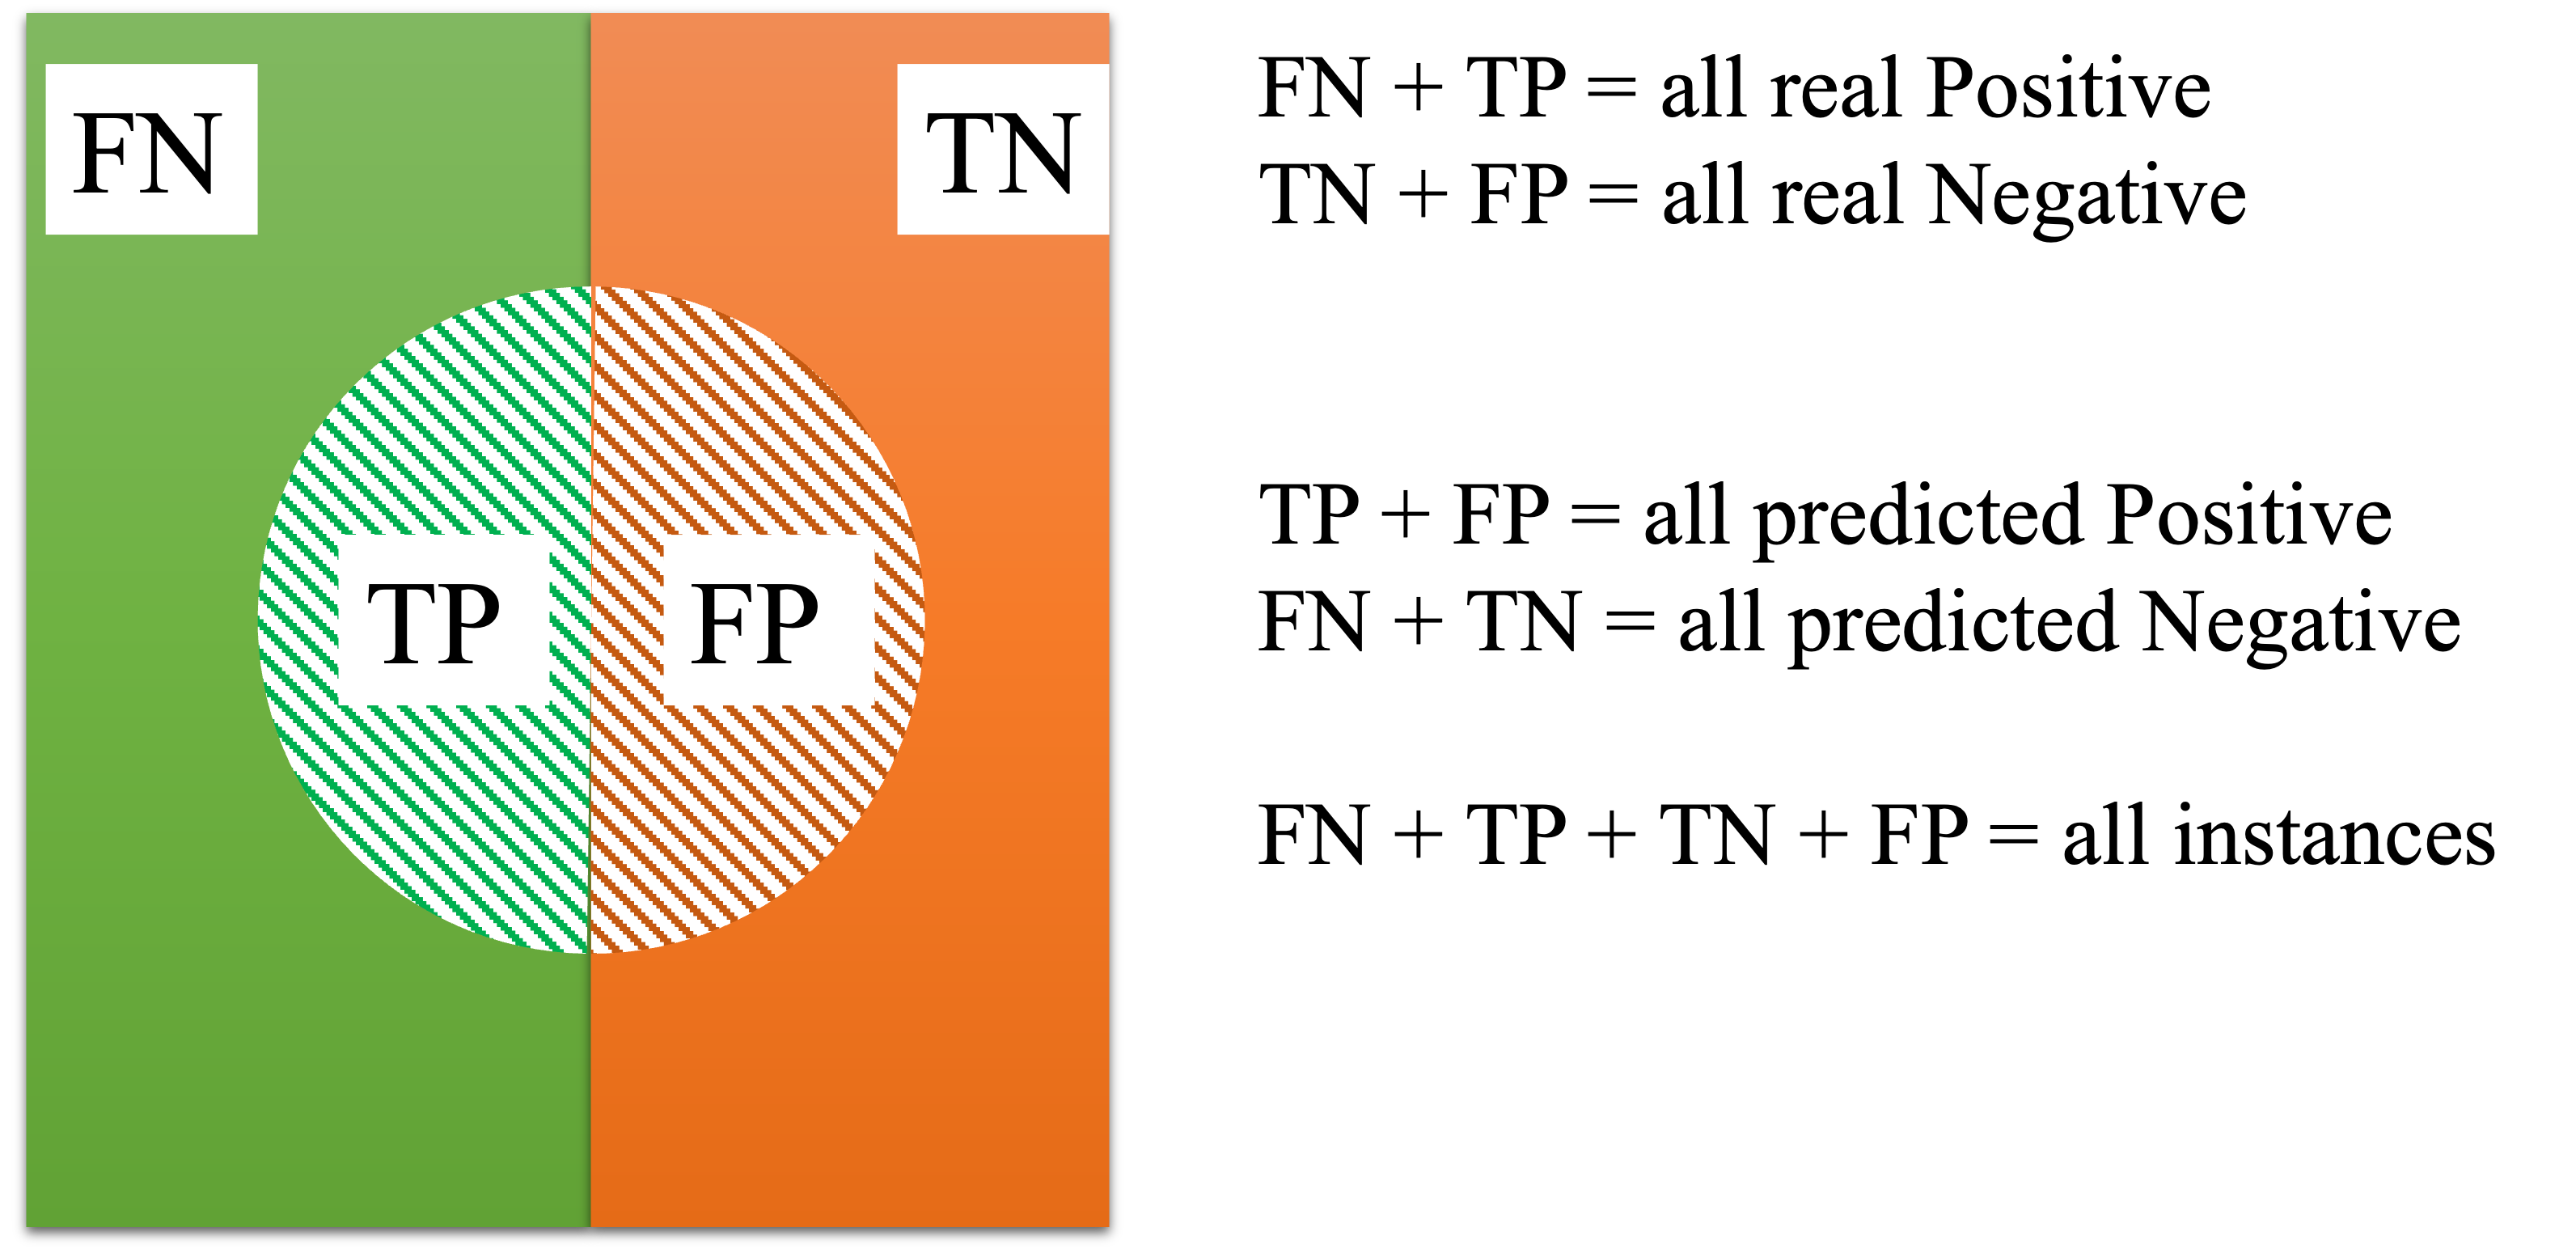
\includegraphics[width=0.78\textwidth]{Topic07fig01.png}
    \caption{Venn-style view of TP, FP, TN, and FN regions.}
  \end{figure}
\end{frame}

\begin{frame}{Overall Accuracy (OA)}
  \justifying
  \[
    OA = \frac{TP + TN}{TP + TN + FP + FN}.
  \]
  \begin{itemize}
    \item OA summarizes global correctness and is easy to communicate.
    \item OA can be misleading when classes are heavily imbalanced.
    \item Always inspect OA together with class-sensitive metrics.
  \end{itemize}
  \vspace{0.3em}
  {\footnotesize Source: \href{https://developers.google.com/machine-learning/crash-course/classification/accuracy-precision-recall}{Google ML Crash Course}}
\end{frame}

\begin{frame}{Precision and Recall: Definitions}
  \justifying
  \[
    \mathrm{Precision} = \frac{TP}{TP + FP}, \qquad
    \mathrm{Recall} = \frac{TP}{TP + FN}.
  \]
  \begin{itemize}
    \item Precision answers: \emph{When we predict positive, how often are we correct?}
    \item Recall answers: \emph{Among actual positives, how many do we detect?}
    \item Precision and recall usually trade off as threshold changes.
  \end{itemize}
  \vspace{0.3em}
  {\footnotesize Source: \href{https://en.wikipedia.org/wiki/Precision_and_recall}{Precision and Recall}}
\end{frame}

\begin{frame}{Precision-Recall Trade-off in Practice}
  \justifying
  \begin{itemize}
    \item Raising a decision threshold often increases precision but decreases recall.
    \item Lowering the threshold usually captures more positives but increases false alarms.
    \item Domain costs determine which side of the trade-off is preferred.
  \end{itemize}
  \begin{examplebox}{Typical Preferences}
    \begin{itemize}
      \item Medical screening: prioritize recall to minimize missed cases.
      \item Fraud filtering: prioritize precision when false alarms are expensive.
    \end{itemize}
  \end{examplebox}
\end{frame}

\begin{frame}{F1 Score and Balanced Detection}
  \justifying
  \[
    F1 = 2\cdot\frac{\mathrm{Precision}\cdot\mathrm{Recall}}{\mathrm{Precision}+\mathrm{Recall}}.
  \]
  \begin{itemize}
    \item F1 is the harmonic mean, so it penalizes imbalance between precision and recall.
    \item A high F1 requires both metrics to be reasonably strong.
    \item F1 is useful when positive detection quality is the primary concern.
  \end{itemize}
  \vspace{0.3em}
  {\footnotesize Source: \href{https://scikit-learn.org/stable/modules/generated/sklearn.metrics.f1_score.html}{scikit-learn f1\_score}}
\end{frame}

\begin{frame}{Worked Example: Spam Detection}
  \justifying

  A common application in machine learning is detecting spam emails. Suppose that in a test set:
\begin{enumerate}
    \item A classification model predicts 100 emails as spam, of which 80 are true positives and 20 are false positives.
    \item The model misses 80 spam emails (i.e., 80 false negatives).
\end{enumerate}

  \[
    \mathrm{Precision} = \frac{80}{80+20}=0.8, \qquad
    \mathrm{Recall} = \frac{80}{80+80}=0.5.
  \]
  \[
    F1 = 2\cdot\frac{0.8\cdot0.5}{0.8+0.5}\approx0.62.
  \]
  \begin{itemize}
    \item Interpretation: predictions labeled as spam are often correct.
    \item Limitation: many true spam messages are still missed.
  \end{itemize}
\end{frame}

\begin{frame}{Specificity and False Positive Rate}
  \justifying
  \[
    \mathrm{Specificity} = \frac{TN}{TN+FP}, \qquad
    1-\mathrm{Specificity} = \frac{FP}{TN+FP}.
  \]
  \begin{itemize}
    \item Specificity emphasizes correctness on the negative class.
    \item $1-\mathrm{Specificity}$ is the false positive rate (FPR), central in ROC analysis.
    \item Sensitivity (recall) and specificity together characterize detection behavior.
  \end{itemize}
\end{frame}

\begin{frame}{Worked Example: Specificity}
  \justifying
  Assume $TN+FP=200$ non-spam emails and $FP=20$.
  \[
    TN=180, \qquad \mathrm{Specificity}=\frac{180}{180+20}=0.9.
  \]
  \begin{itemize}
    \item The classifier rejects non-spam emails correctly 90\% of the time.
    \item High specificity does not guarantee high recall on spam.
  \end{itemize}
\end{frame}

\begin{frame}{Binary Metrics Summary}
  \justifying
  \begin{itemize}
    \item TP/FP/TN/FN are the primitive counts that drive all binary metrics.
    \item Precision, recall, specificity, and OA capture different error patterns.
    \item F1 is a compact score when precision and recall are jointly important.
    \item Good reporting shows multiple metrics instead of a single headline number.
  \end{itemize}
\end{frame}

\section{Random-guess Classifier Baseline}

\begin{frame}{Random-guess Geometry}
  \justifying
  \begin{figure}[ht]
    \centering
    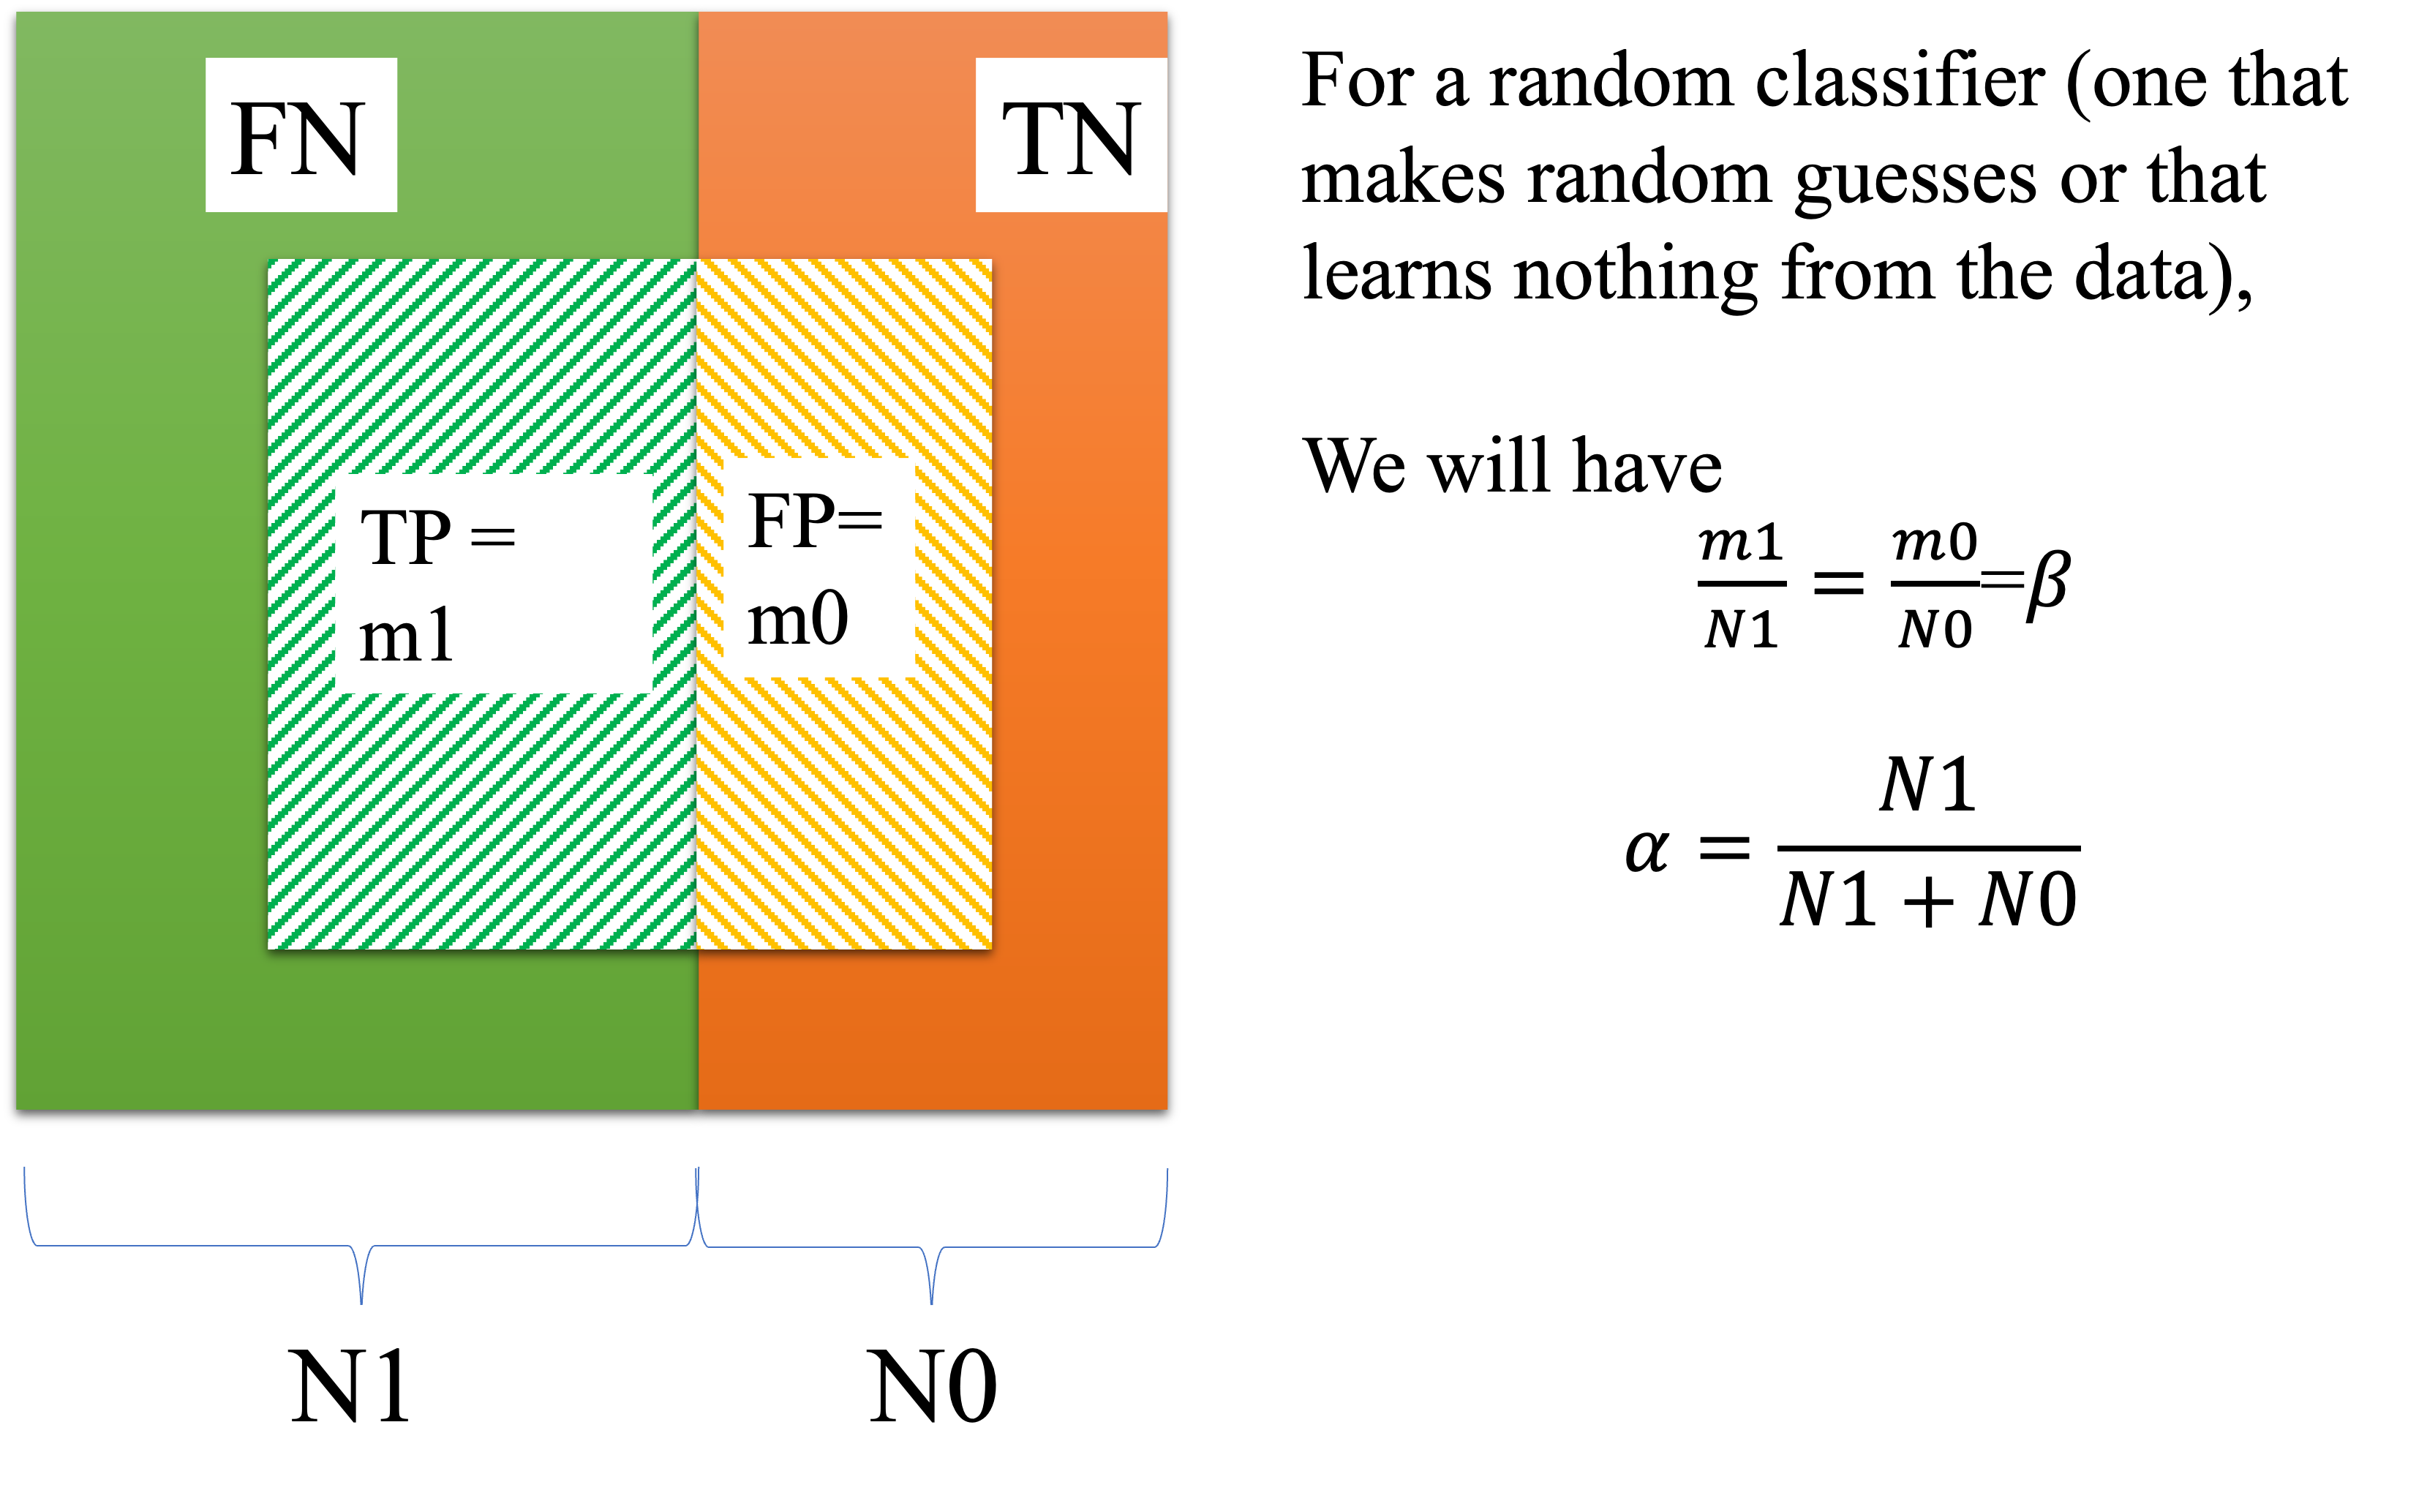
\includegraphics[width=0.78\textwidth]{Topic07fig02.png}
    \caption{Venn interpretation of random guessing behavior.}
  \end{figure}
\end{frame}

\begin{frame}{RGC Setup and Notation}
  \justifying
  \begin{itemize}
    \item Let $N_1$ be actual positives and $N_0$ actual negatives.
    \item Let $m_1$ be correct positive guesses (TP) and $m_0$ incorrect positive guesses (FP).
    \item Random assignment implies matching class-ratio behavior:
    \[
      \frac{m_1}{m_0}=\frac{N_1}{N_0}.
    \]
  \end{itemize}
\end{frame}

\begin{frame}{RGC Precision, Recall, and FPR}
  \justifying
  Define
  \[
    \beta = \frac{m_1}{N_1}=\frac{m_0}{N_0},
    \qquad
    \alpha = \frac{N_1}{N_1+N_0}.
  \]
  Then
  \[
    \mathrm{Precision}=\alpha,
    \quad
    \mathrm{Recall}=\beta,
    \quad
    1-\mathrm{Specificity}=\beta.
  \]
  \begin{itemize}
    \item Precision is constant and equals class prevalence.
    \item Recall and FPR vary together with threshold behavior.
  \end{itemize}
\end{frame}

\begin{frame}{Implications of the Random Baseline}
  \justifying
  \begin{itemize}
    \item On ROC space, random guessing forms the diagonal from $(0,0)$ to $(1,1)$.
    \item On PR space, random guessing forms a horizontal line at prevalence $\alpha$.
    \item Learned models should produce ROC/PR curves above these baseline references.
  \end{itemize}
\end{frame}

\section{One-hot Encoding and Softmax}

\begin{frame}{Why Integer Labels Are Not Enough}
  \justifying
  \begin{itemize}
    \item Integer labels like $1,2,3$ may imply false ordinal relationships between classes.
    \item Multi-class learning requires categorical representation without distance assumptions.
    \item One-hot encoding preserves identity while avoiding artificial rank structure.
  \end{itemize}
\end{frame}

\begin{frame}{One-hot Encoding Definition}
  \justifying
  \begin{conceptbox}{One-of-K Representation}
    For $K$ classes, each label becomes a vector in $\{0,1\}^K$ with exactly one entry equal to 1.
  \end{conceptbox}
  \begin{itemize}
    \item Class index identifies which position is active.
    \item Vector sum is always one, matching probability simplex structure.
  \end{itemize}
\end{frame}

\begin{frame}{One-hot Example for Three Classes}
  \justifying
  \[
    \mathbf{c}(1)=[1,0,0],\quad
    \mathbf{c}(2)=[0,1,0],\quad
    \mathbf{c}(3)=[0,0,1].
  \]
  \begin{itemize}
    \item Exactly one active component identifies each class.
    \item No class appears numerically larger or closer than another.
  \end{itemize}
  \vspace{0.3em}
  {\footnotesize Source: \href{https://scikit-learn.org/stable/modules/generated/sklearn.preprocessing.OneHotEncoder.html}{scikit-learn OneHotEncoder}}
\end{frame}

\begin{frame}{Matrix View of Encoded Labels}
  \justifying
  \begin{itemize}
    \item With $N$ samples and $K$ classes, encoded labels form $\mathbf{C}\in\mathbb{R}^{N\times K}$.
    \item Class counts are recovered by column sums:
    \[
      N_k = \sum_n C_{n,k}.
    \]
    \item This representation is computationally convenient for batched training.
  \end{itemize}
\end{frame}

\begin{frame}{From Sigmoid to Softmax}
  \justifying
  \begin{itemize}
    \item Binary logistic models map one score to one probability via sigmoid.
    \item Multi-class models require normalized probabilities across $K$ classes.
    \item Softmax is the standard transformation from scores to a categorical distribution.
  \end{itemize}
\end{frame}

\begin{frame}{Softmax Definition and Properties}
  \justifying
  \[
    \sigma_i(\bm{z})=\frac{e^{z_i}}{\sum_{j=1}^K e^{z_j}},
    \qquad
    \sum_{i=1}^K \sigma_i(\bm{z})=1.
  \]
  \begin{itemize}
    \item Larger $z_i$ values increase class $i$ probability monotonically.
    \item Output is interpretable as a probability simplex point.
    \item In $K=2$, softmax reduces to sigmoid-equivalent behavior.
  \end{itemize}
  \vspace{0.3em}
  {\footnotesize Source: \href{https://www.tensorflow.org/api_docs/python/tf/keras/layers/Softmax}{TensorFlow Softmax}}
\end{frame}

\begin{frame}{Prediction Rule with Softmax}
  \justifying
  \[
    \hat{k}=\arg\max_i\ \sigma_i(\bm{z}),
    \qquad
    c(\hat{k})=1.
  \]
  \begin{itemize}
    \item Prediction chooses the highest posterior score among classes.
    \item Confidence calibration may still require additional post-processing.
  \end{itemize}
  \begin{warningbox}{Operational Note}
    High softmax probability does not always imply calibrated real-world confidence.
  \end{warningbox}
\end{frame}

\section{One-vs-All and One-vs-Rest}

\begin{frame}{Why Decomposition Strategies Exist}
  \justifying
  \begin{itemize}
    \item Some classifiers are naturally binary (for example, standard SVM formulations).
    \item Decomposition builds multi-class capability from binary decision modules.
    \item Strategy choice affects computational cost and decision aggregation behavior.
  \end{itemize}
\end{frame}

\begin{frame}{One-vs-All (OvA) Strategy}
  \justifying
  \begin{conceptbox}{OvA Construction}
    \begin{itemize}
      \item Train $K$ binary classifiers.
      \item Classifier $i$ treats class $i$ as positive and all others as negative.
      \item At inference, choose class with highest decision score.
    \end{itemize}
  \end{conceptbox}
\end{frame}

\begin{frame}{OvA Example for Three Classes}
  \justifying
  \begin{itemize}
    \item Classifier 1: class 1 vs classes 2 and 3.
    \item Classifier 2: class 2 vs classes 1 and 3.
    \item Classifier 3: class 3 vs classes 1 and 2.
  \end{itemize}
  \begin{itemize}
    \item Total models: $K$.
    \item Works well when one class must be distinguished from a broad background.
  \end{itemize}
\end{frame}

\begin{frame}{One-vs-Rest Pairwise Scheme (OvR in Notes)}
  \justifying
  \begin{itemize}
    \item Pairwise decomposition trains one classifier per class pair.
    \item Number of models: $\frac{K(K-1)}{2}$.
    \item Final class is chosen by aggregating pairwise scores or votes.
  \end{itemize}
  \vspace{0.3em}
  {\footnotesize Source: \href{https://scikit-learn.org/stable/modules/multiclass.html}{scikit-learn Multiclass Strategies}}
\end{frame}

\begin{frame}{OvA vs Pairwise: Practical Comparison}
  \justifying
  \begin{table}[ht]
    \centering
    \begin{tabular}{p{3cm}p{7cm}}
      \toprule
      Aspect & Observation \\
      \midrule
      Number of models & OvA: $K$; Pairwise: $K(K-1)/2$ \\
      Training cost & Pairwise can be heavier as $K$ grows \\
      Decision behavior & Pairwise can improve local discrimination \\
      Typical choice & OvA is often simpler and scalable \\
      \bottomrule
    \end{tabular}
  \end{table}
\end{frame}

\begin{frame}{When to Use Which Strategy}
  \justifying
  \begin{itemize}
    \item Prefer OvA for large $K$ and simpler deployment pipelines.
    \item Consider pairwise decomposition when class boundaries are nuanced and close.
    \item Validate both with cross-validation instead of relying on intuition only.
  \end{itemize}
  \vspace{0.3em}
  {\footnotesize Source: \href{https://scikit-learn.org/stable/modules/generated/sklearn.multiclass.OneVsRestClassifier.html}{scikit-learn OneVsRestClassifier}}
\end{frame}

\section{Multi-class Accuracy Measures}

\begin{frame}{Why Multi-class Metrics Need Care}
  \justifying
  \begin{itemize}
    \item In multi-class settings, there is no universal positive class by default.
    \item TP/FP/TN/FN must be defined relative to a selected class $c_i$.
    \item Reporting should include class-wise views and global averages.
  \end{itemize}
\end{frame}

\begin{frame}{Testing Set Notation}
  \justifying
  \[
    \mathcal{D}^{\text{testing}} = \{(\bm{x}_m,c_m)\mid m=1,\ldots,M\},
    \quad c_m\in\{c_1,\ldots,c_K\}.
  \]
  \begin{itemize}
    \item $M$ is the total number of test instances.
    \item $K$ is the number of classes.
    \item We evaluate predictions by comparing $\hat{c}_m$ to $c_m$.
  \end{itemize}
\end{frame}

\begin{frame}{$K\times K$ Confusion Matrix}
  \justifying
  \begin{itemize}
    \item Denote confusion matrix entries by $CF(i,j)$.
    \item Rows represent predicted labels; columns represent true labels.
    \item Total sample count is
    \[
      M=\sum_i\sum_j CF(i,j).
    \]
  \end{itemize}
\end{frame}

\begin{frame}{Three-Class Confusion Matrix Example}
  \justifying
  \begin{table}[ht]
    \centering
    \begin{tabular}{c|ccc}
      \hline
      Predicted $\backslash$ True & A & B & C \\
      \hline
      A & 8 & 0 & 3 \\
      B & 2 & 4 & 1 \\
      C & 0 & 0 & 12 \\
      \hline
    \end{tabular}
  \end{table}
  \begin{itemize}
    \item Diagonal entries are correct predictions.
    \item Off-diagonal entries are misclassifications.
  \end{itemize}
\end{frame}

\begin{frame}{Reading Row and Column Totals}
  \justifying
  \begin{itemize}
    \item $\sum_{j'}CF(i,j')$: instances predicted as class $i$ (row total).
    \item $\sum_{i'}CF(i',j)$: instances truly belonging to class $j$ (column total).
    \item $\sum_i CF(i,i)$: total number of correctly classified samples.
  \end{itemize}
\end{frame}

\begin{frame}{Class-wise TP, FP, FN, TN}
  \justifying
  For selected class $c_i$:
  \begin{itemize}
    \item $TP_i = CF(i,i)$.
    \item $FP_i = \sum_{j'\neq i} CF(i,j')$.
    \item $FN_i = \sum_{i'\neq i} CF(i',i)$.
    \item $TN_i = \sum_{i'}\sum_{j'}CF(i',j') - \sum_{j'}CF(i,j') - \sum_{i'}CF(i',i) + CF(i,i)$.
  \end{itemize}
\end{frame}

\begin{frame}{Class-wise Precision and Recall}
  \justifying
  \[
    \mathrm{Precision}_i = \frac{TP_i}{TP_i+FP_i},
    \qquad
    \mathrm{Recall}_i = \frac{TP_i}{TP_i+FN_i}.
  \]
  \begin{itemize}
    \item Each class gets its own precision/recall pair.
    \item Weak minority-class recall can be hidden by majority-class performance.
  \end{itemize}
\end{frame}

\begin{frame}{Overall Accuracy and Error Rate}
  \justifying
  \[
    OA = \frac{\sum_i CF(i,i)}{\sum_i\sum_j CF(i,j)},
    \qquad
    ER = 1 - OA.
  \]
  \begin{itemize}
    \item OA and ER provide compact global summaries.
    \item They should be accompanied by class-wise metrics in imbalanced datasets.
  \end{itemize}
\end{frame}

\begin{frame}{Macro, Micro, and Weighted Averages}
  \justifying
  \begin{itemize}
    \item Macro average: unweighted mean across classes (treats classes equally).
    \item Micro average: global count-based aggregation (favors large classes).
    \item Weighted average: class-wise scores weighted by class support.
  \end{itemize}
  \vspace{0.3em}
  {\footnotesize Sources: \href{https://scikit-learn.org/stable/modules/model_evaluation.html}{Model Evaluation}, \href{https://scikit-learn.org/stable/modules/generated/sklearn.metrics.classification_report.html}{classification\_report}}
\end{frame}

\begin{frame}{Interpreting Averages in Reports}
  \justifying
  \begin{examplebox}{Typical Diagnostic Pattern}
    \begin{itemize}
      \item High micro-F1 but low macro-F1 indicates minority classes are underperforming.
      \item Similar macro and weighted scores suggest balanced class behavior.
      \item Large spread in per-class F1 values signals targeted model refinement is needed.
    \end{itemize}
  \end{examplebox}
\end{frame}

\begin{frame}{Multi-class Evaluation Checklist}
  \justifying
  \begin{itemize}
    \item Inspect confusion matrix structure before looking at aggregate metrics.
    \item Report per-class precision/recall/F1 with support counts.
    \item Include macro and micro averages to expose imbalance effects.
    \item Validate metrics under cross-validation or repeated splits when feasible.
  \end{itemize}
\end{frame}

\section{Advanced Visual Analytics}

\begin{frame}{ROC Curves: Core Definition}
  \justifying
  \begin{itemize}
    \item ROC plots true positive rate (TPR) against false positive rate (FPR).
    \item Each point corresponds to one decision threshold.
    \item Better models push the curve toward the top-left corner.
  \end{itemize}
  \[
    TPR=\frac{TP}{TP+FN}, \qquad FPR=\frac{FP}{FP+TN}.
  \]
\end{frame}

\begin{frame}{ROC Visualization}
  \justifying
  \begin{figure}[ht]
    \centering
    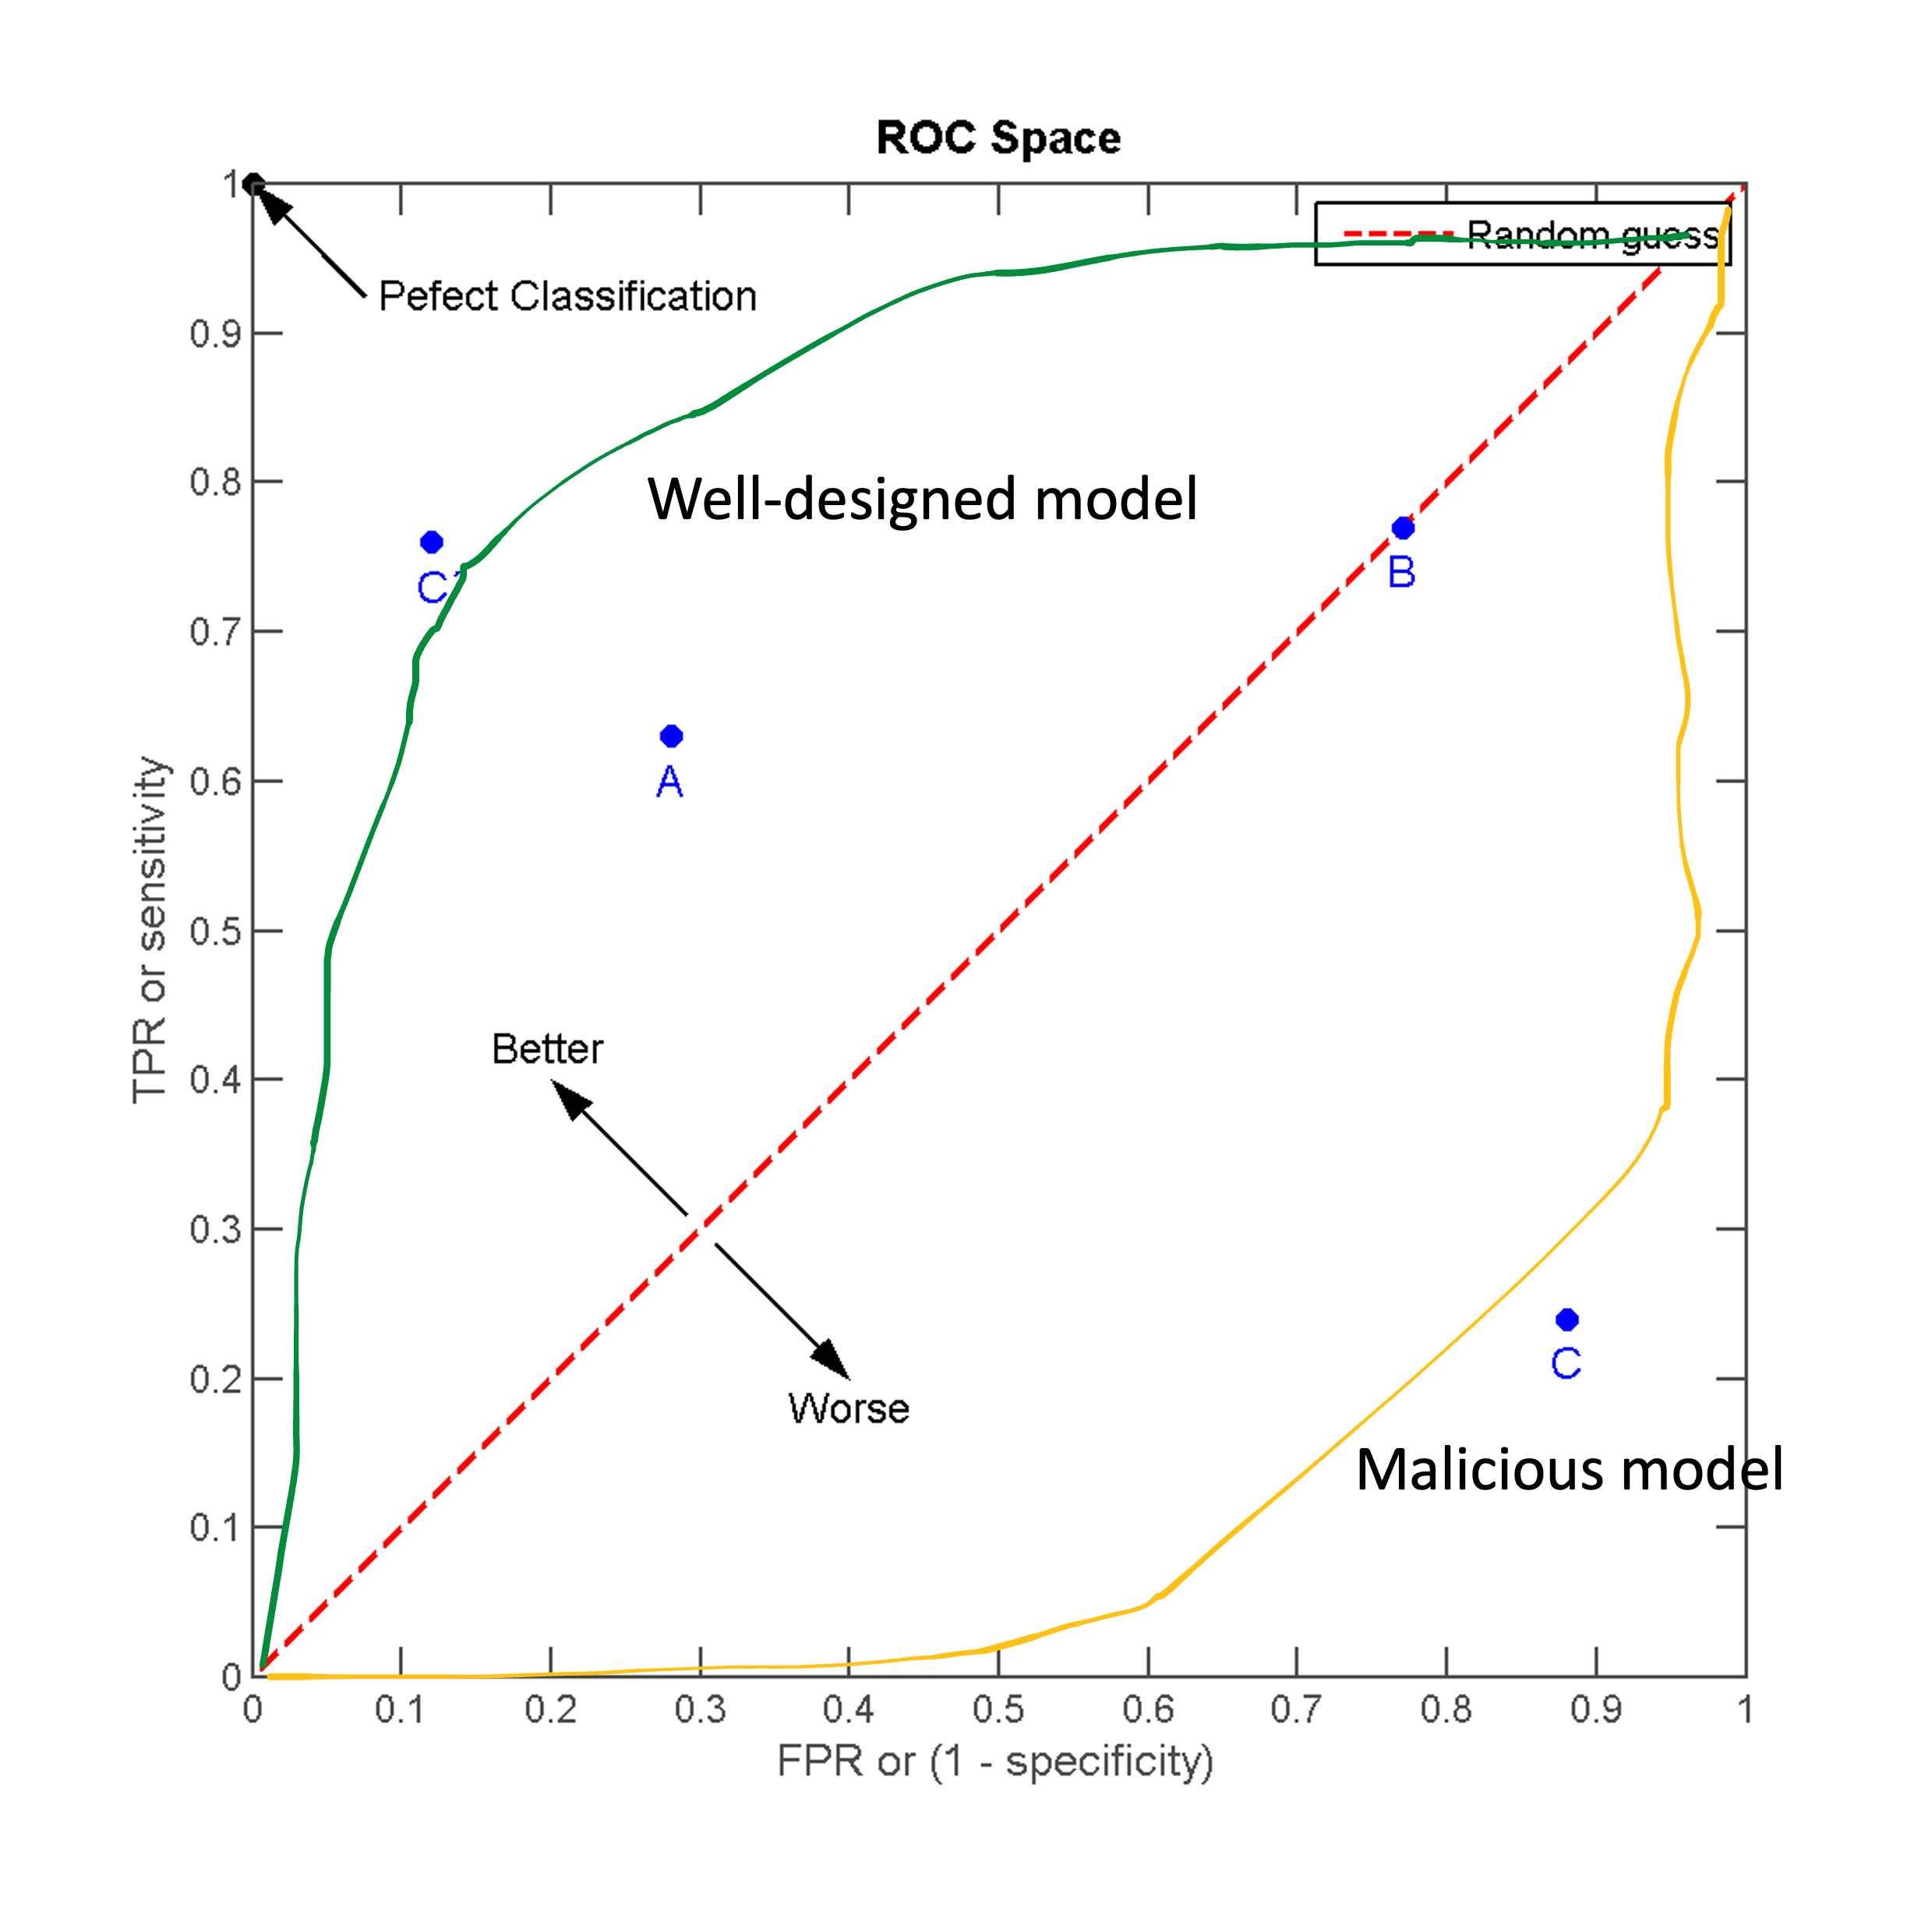
\includegraphics[width=0.70\textwidth]{Topic08fig01.png}
    \caption{ROC curve with random baseline and model capacity contrast.}
  \end{figure}
\end{frame}

\begin{frame}{AUC for ROC Curves}
  \justifying
  \[
    AUC = \int ROC(\alpha)\,d\alpha.
  \]
  \begin{itemize}
    \item $AUC=1$ indicates perfect ranking behavior.
    \item $AUC=0.5$ corresponds to random guessing.
    \item Values below 0.5 indicate systematically reversed ranking.
  \end{itemize}
  \vspace{0.3em}
  {\footnotesize Sources: \href{https://scikit-learn.org/stable/modules/generated/sklearn.metrics.roc_curve.html}{roc\_curve}, \href{https://scikit-learn.org/stable/modules/generated/sklearn.metrics.roc_auc_score.html}{roc\_auc\_score}}
\end{frame}

\begin{frame}{When ROC Can Mislead}
  \justifying
  \begin{warningbox}{Class Imbalance Caveat}
    \begin{itemize}
      \item In highly imbalanced datasets, large TN counts can make FPR look deceptively small.
      \item A model can appear strong on ROC while still producing weak precision.
      \item Pair ROC with PR analysis when positives are rare.
    \end{itemize}
  \end{warningbox}
\end{frame}

\begin{frame}{Precision-Recall (PR) Curves}
  \justifying
  \begin{itemize}
    \item PR curves plot precision as a function of recall over thresholds.
    \item They directly emphasize positive-class retrieval quality.
    \item They are often more informative than ROC under severe imbalance.
  \end{itemize}
\end{frame}

\begin{frame}{PR Curve Visualization}
  \justifying
  \begin{figure}[ht]
    \centering
    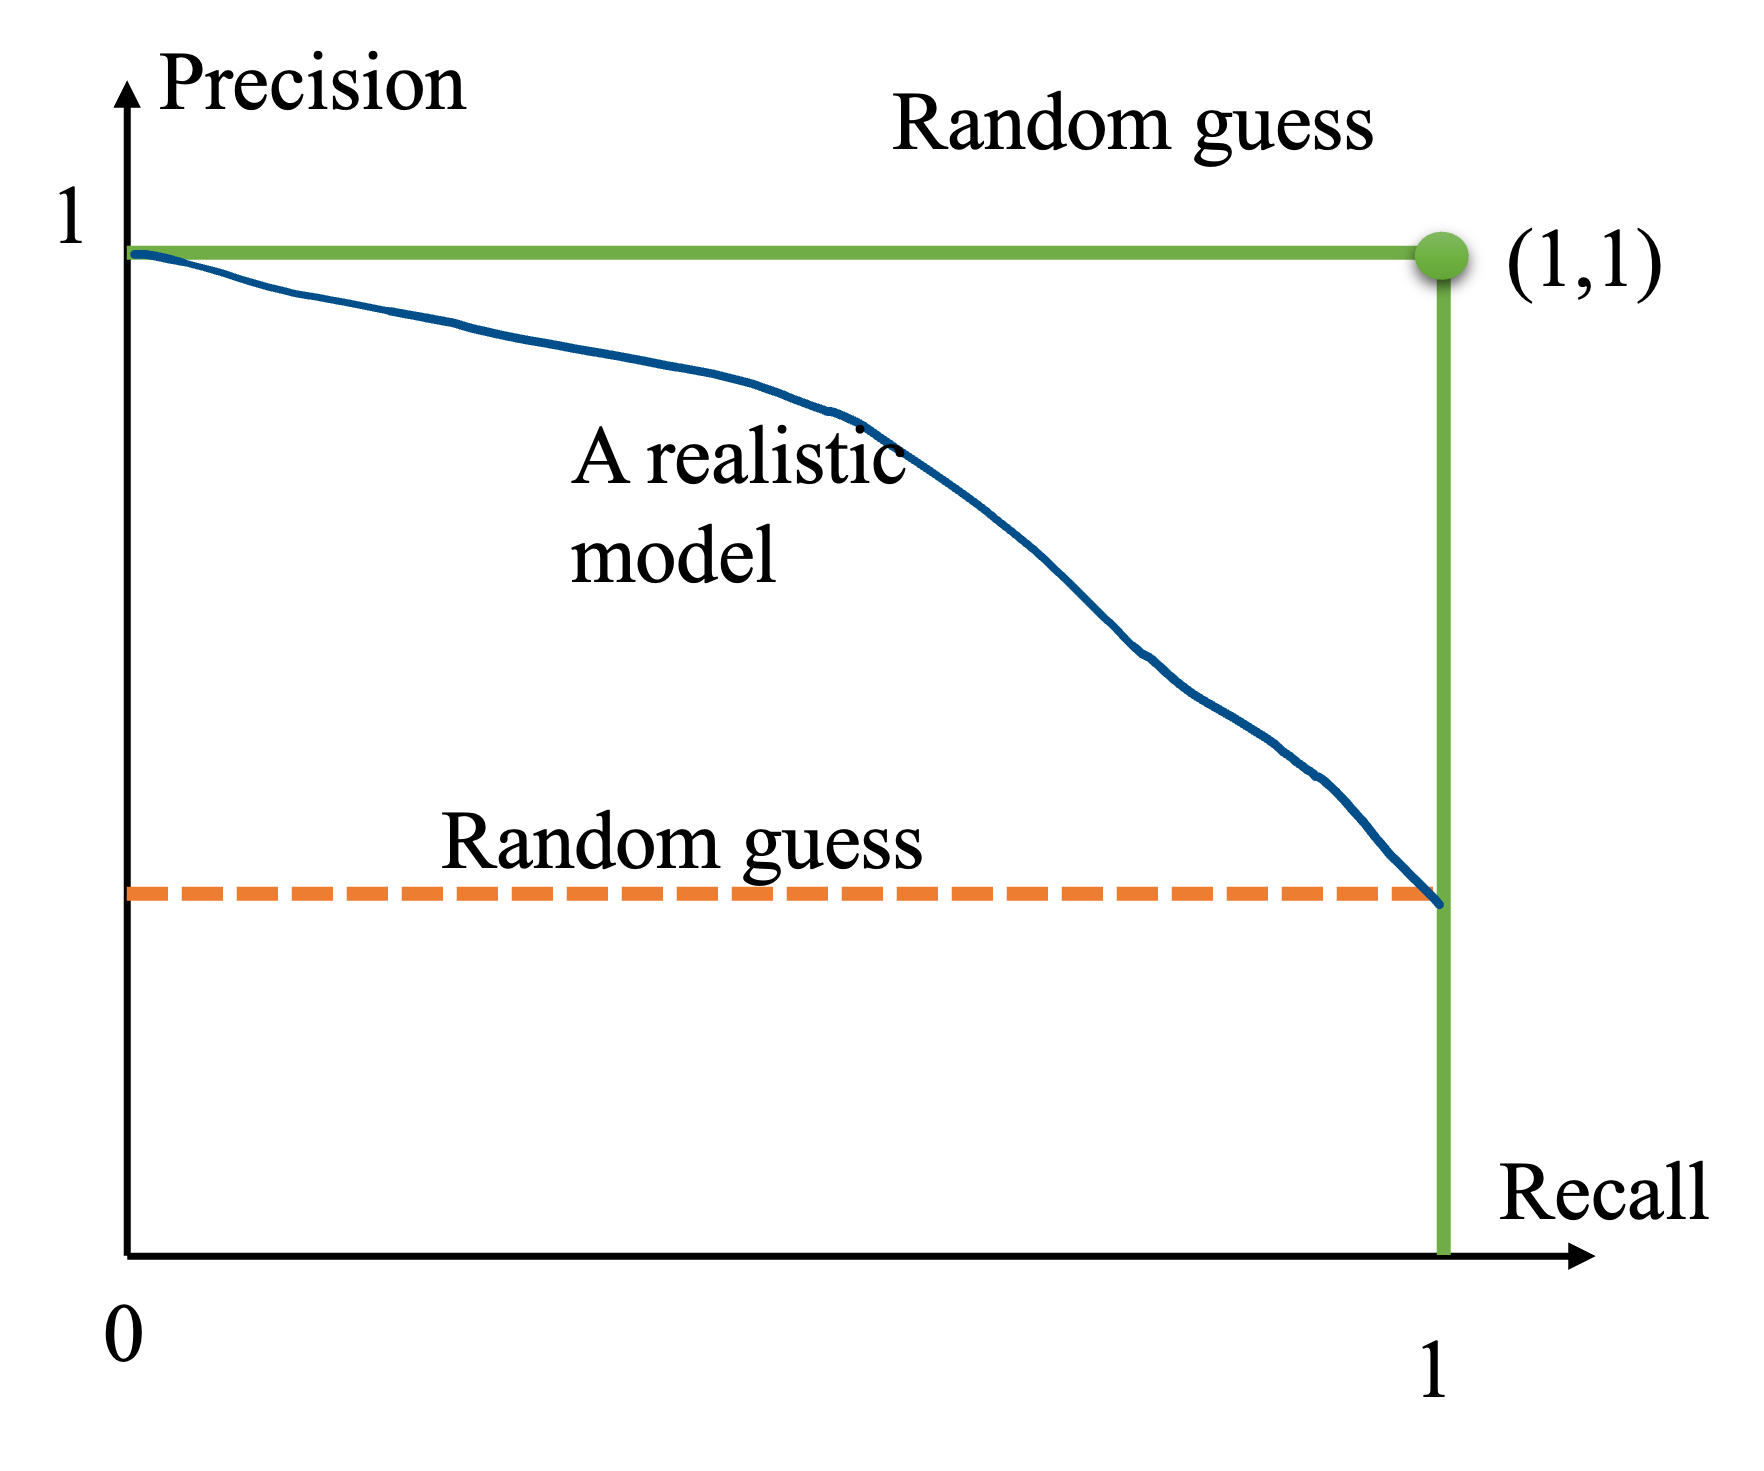
\includegraphics[width=0.64\textwidth]{Topic08fig02.png}
    \caption{Precision-recall curve and threshold-dependent trade-off.}
  \end{figure}
\end{frame}

\begin{frame}{Reading PR Curves and AUC-PR}
  \justifying
  \begin{itemize}
    \item Better models keep precision high while recall increases.
    \item Random baseline appears as a horizontal line at prevalence.
    \item AUC-PR summarizes curve quality on $[0,1]$, with larger values preferred.
  \end{itemize}
  \vspace{0.3em}
  {\footnotesize Sources: \href{https://scikit-learn.org/stable/modules/generated/sklearn.metrics.precision_recall_curve.html}{precision\_recall\_curve}, \href{https://scikit-learn.org/stable/auto_examples/model_selection/plot_precision_recall.html}{PR Example}}
\end{frame}

\section{Summary and Resources}

\begin{frame}{Topic 7 Summary (Part 1)}
  \justifying
  \begin{itemize}
    \item Binary evaluation starts from TP, FP, TN, and FN, then extends to precision, recall, specificity, and F1.
    \item Random-guess baselines provide non-negotiable context for ROC and PR interpretation.
    \item One-hot encoding and softmax provide the standard probabilistic interface for multi-class outputs.
  \end{itemize}
\end{frame}

\begin{frame}{Topic 7 Summary (Part 2)}
  \justifying
  \begin{itemize}
    \item OvA and pairwise decomposition adapt binary learners to multi-class settings.
    \item Multi-class confusion matrices support class-wise and averaged metrics.
    \item Robust reporting combines global scores, per-class behavior, and threshold curves.
  \end{itemize}
\end{frame}

\begin{frame}{What to Practice Next}
  \justifying
  \begin{itemize}
    \item Compute macro/micro/weighted F1 on the same model and explain discrepancies.
    \item Plot ROC and PR curves on imbalanced and balanced datasets for contrast.
    \item Compare softmax multi-class training against OvA decomposition on one dataset.
    \item Document how threshold tuning changes precision-recall trade-offs.
  \end{itemize}
\end{frame}

\begin{frame}{External Resources (1/2)}
  \justifying
  \footnotesize
  \begin{itemize}
    \item \href{https://scikit-learn.org/stable/modules/model_evaluation.html}{scikit-learn: Model Evaluation and Scoring}
    \item \href{https://scikit-learn.org/stable/modules/generated/sklearn.metrics.f1_score.html}{scikit-learn: f1\_score}
    \item \href{https://scikit-learn.org/stable/modules/generated/sklearn.metrics.classification_report.html}{scikit-learn: classification\_report}
    \item \href{https://developers.google.com/machine-learning/crash-course/classification/accuracy-precision-recall}{Google ML Crash Course: Accuracy, Precision, Recall}
    \item \href{https://en.wikipedia.org/wiki/Precision_and_recall}{Wikipedia: Precision and Recall}
    \item \href{https://scikit-learn.org/stable/modules/generated/sklearn.metrics.roc_curve.html}{scikit-learn: roc\_curve}
  \end{itemize}
\end{frame}

\begin{frame}{External Resources (2/2)}
  \justifying
  \footnotesize
  \begin{itemize}
    \item \href{https://scikit-learn.org/stable/modules/generated/sklearn.metrics.roc_auc_score.html}{scikit-learn: roc\_auc\_score}
    \item \href{https://scikit-learn.org/stable/auto_examples/model_selection/plot_roc.html}{scikit-learn: ROC Example}
    \item \href{https://scikit-learn.org/stable/modules/generated/sklearn.metrics.precision_recall_curve.html}{scikit-learn: precision\_recall\_curve}
    \item \href{https://scikit-learn.org/stable/auto_examples/model_selection/plot_precision_recall.html}{scikit-learn: PR Example}
    \item \href{https://scikit-learn.org/stable/modules/generated/sklearn.preprocessing.OneHotEncoder.html}{scikit-learn: OneHotEncoder}
    \item \href{https://www.tensorflow.org/api_docs/python/tf/keras/layers/Softmax}{TensorFlow: Softmax Layer}
    \item \href{https://scikit-learn.org/stable/modules/multiclass.html}{scikit-learn: Multiclass and Multioutput}
    \item \href{https://scikit-learn.org/stable/modules/generated/sklearn.multiclass.OneVsRestClassifier.html}{scikit-learn: OneVsRestClassifier}
  \end{itemize}
\end{frame}

\end{document}
